% -------------------------------------------------------
%  Section 8: Reproduction on BIG 2015
% -------------------------------------------------------
\clearpage
\section{بازپیاده‌سازی و بازتولید نتایج روی \lr{BIG 2015}}
\label{sec:repro}

\subsection{پیاده‌سازی}
نشانی مخزنی که مقاله اعلام کرده در دسترس نیست (\S\ref{sec:identity})، پس بازتولید تنها از روی توصیف متن ممکن بود؛ این با هدف فاز سوم درس نیز هم‌خوان است که بازنویسی مستقل روش را می‌خواهد. کل خط لوله را از ابتدا در \lr{PyTorch} پیاده‌سازی کردیم و آن را به‌صورت یک بسته پایتونی با رابط خط فرمان سازمان دادیم. این پیاده‌سازی پنج مؤلفه دارد: دریافت و آماده‌سازی داده، پیش‌پردازش و تولید بازنمایی‌های \lr{S1} تا \lr{S5}، ساخت مدل، آموزش و ارزیابی، و تولید فایل ارسال به کگل.

یک تصمیم طراحی که بعداً برای فاز چهارم تعیین‌کننده شد، جدا کردن کامل فرادادهٔ مجموعه‌داده از منطق برنامه بود: کلاس‌ها، بخش‌های هدف، تعریف کانال‌ها و فهرست پیکربندی‌ها همگی در یک فایل \kd{JSON} توصیف می‌شوند؛ آزمایش‌های این بخش با پیکربندی \kd{big2015.json} اجرا شده‌اند. به این ترتیب افزودن یک مجموعه‌داده تازه با قالب و معناشناسی بخش‌های متفاوت، بدون دست زدن به کد آموزش ممکن شد.

\subsection{میزان وفاداری به مقاله و انحراف‌های ناگزیر}
ابرپارامتر‌های جدول \ref{tab:hyper}، دو معماری، پنج طرح داده، عرض پایه \num{۱۰۲۴} برای \lr{S4} و \lr{S5}، قاعده نگاشت بایت‌های \kd{??} به صفر و اندازه نهایی $224 \times 224$ همگی عیناً از مقاله گرفته شده‌اند. پروتکل ارزیابی نیز همان است: پیش‌بینی روی \num{۱۰٬۸۷۳} نمونه آزمون بدون برچسب و ارسال به سرور کگل برای دریافت نمره عمومی و خصوصی.

سه انحراف ناگزیر وجود دارد که برای شفافیت ثبت می‌شوند. نخست، سیاست کانال‌های غایب که در مقاله مشخص نشده و ما آن را با کانال تمام‌صفر پیاده کردیم. دوم، بهنجارسازی کانال‌های چهارم و پنجم که میانگین \num{۰٫۵} و انحراف معیار \num{۰٫۲۲۵} می‌گیرند، چون \lr{ImageNet} تنها برای سه کانال مقدار مرجع دارد. سوم، فعال بودن دقت مختلط\pn{Automatic Mixed Precision} برای کاهش زمان اجرا. بذر تصادفی را روی \num{۴۲} ثابت کردیم؛ مقاله بذری گزارش نکرده است.

\subsection{نتایج}
جدول \ref{tab:bigrepro} هر ۲۰ پیکربندی جدول ۵ مقاله را در کنار نتایج ما قرار می‌دهد و شکل \ref{fig:logloss} همین داده را به‌صورت بصری نشان می‌دهد. ستون آخر، اجرای کوتاه‌شده با ۱۰ دوره است که برای سنجش حساسیت به بودجه آموزش انجام دادیم.

\begin{table}[!ht]
    \centering
    \scriptsize
    \caption{بازتولید ۲۰ پیکربندی مقاله روی \lr{BIG 2015}؛ همه اعداد زیان لگاریتمی چندکلاسه‌اند (کمتر بهتر است)}
    \label{tab:bigrepro}
    \begin{tabular}{|l|l|c|c|c|c|c|}
    \hline
    \textbf{مدل} & \textbf{پیکربندی} & \textbf{مقاله} & \textbf{ما، عمومی} & \textbf{ما، خصوصی} & \textbf{اختلاف} & \textbf{ما، ۱۰ دوره} \\ \hline
    \lr{VGG16} & \lr{S1} & \num{۰٫۰۴۰۱} & \num{۰٫۰۵۲۳۴} & \num{۰٫۰۵۳۳۷} & \num{+۰٫۰۱۳۳} & \num{۰٫۰۴۴۲۳} \\ \hline
     & \lr{S2} & \num{۰٫۰۵۴۷} & \num{۰٫۰۵۳۱۴} & \num{۰٫۰۵۰۴۶} & \num{−۰٫۰۰۴۲} & \num{۰٫۰۴۶۲۷} \\ \hline
     & \lr{S3} & \num{۰٫۰۴۱۱} & \num{۰٫۰۳۵۴۰} & \num{۰٫۰۴۳۶۵} & \num{+۰٫۰۰۲۶} & \num{۰٫۰۴۴۸۹} \\ \hline
     & \lr{S4 (.text + .rdata + .rsrc)} & \num{۰٫۰۵۷۷} & \num{۰٫۰۹۱۵۲} & \num{۰٫۰۹۲۲۶} & \num{+۰٫۰۳۴۶} & \num{۰٫۰۸۸۶۱} \\ \hline
     & \lr{S5 (imgs-1024 + .text + .rsrc)} & \num{۰٫۰۵۲۱} & \num{۰٫۰۶۱۰۱} & \num{۰٫۰۵۷۰۹} & \num{+۰٫۰۰۵۰} & \num{۰٫۰۵۱۲۸} \\ \hline
     & \lr{S5 (.text + .rdata + .rsrc)} & \num{۰٫۰۸۸۹} & \num{۰٫۲۲۸۹۴} & \num{۰٫۲۱۸۸۳} & \num{+۰٫۱۲۹۹} & \num{۰٫۱۲۲۹۵} \\ \hline
    \lr{ResNet50} & \lr{S1} & \num{۰٫۰۳۱۶} & \num{۰٫۰۳۴۷۷} & \num{۰٫۰۳۶۰۱} & \num{+۰٫۰۰۴۴} & \num{۰٫۰۳۷۳۵} \\ \hline
     & \lr{S2} & \num{۰٫۰۳۳۰} & \num{۰٫۰۳۳۳۲} & \num{۰٫۰۳۹۱۶} & \num{+۰٫۰۰۶۲} & \num{۰٫۰۴۶۴۱} \\ \hline
     & \lr{S3} & \num{۰٫۰۲۶۵} & \num{۰٫۰۳۲۷۹} & \num{۰٫۰۳۴۴۶} & \num{+۰٫۰۰۸۰} & \num{۰٫۰۳۸۰۰} \\ \hline
     & \lr{S4 (.rdata + .data + .rsrc)} & \num{۰٫۰۵۸۷} & \num{۰٫۱۰۹۱۴} & \num{۰٫۰۸۵۵۹} & \num{+۰٫۰۲۶۹} & \num{۰٫۰۸۷۴۷} \\ \hline
     & \lr{S4 (.text + .data + .rsrc)} & \num{۰٫۰۳۸۳} & \num{۰٫۰۸۷۶۱} & \num{۰٫۰۸۲۴۴} & \num{+۰٫۰۴۴۱} & \num{۰٫۰۸۷۶۱} \\ \hline
     & \lr{S4 (.text + .rdata + .data)} & \num{۰٫۰۴۵۲} & \num{۰٫۱۱۷۹۶} & \num{۰٫۰۹۳۷۱} & \num{+۰٫۰۴۸۵} & \num{۰٫۰۹۷۹۳} \\ \hline
     & \lr{S4 (.text + .rdata + .data + .rsrc)} & \num{۰٫۰۳۶۴} & \num{۰٫۰۹۵۲۸} & \num{۰٫۰۸۳۸۸} & \num{+۰٫۰۴۷۵} & \num{۰٫۰۷۱۸۵} \\ \hline
     & \lr{S4 (.text + .rdata + .rsrc)} & \num{۰٫۰۳۲۰} & \num{۰٫۱۰۸۲۵} & \num{۰٫۰۸۴۱۰} & \num{+۰٫۰۵۲۱} & \num{۰٫۰۸۲۹۷} \\ \hline
     & \lr{S5 (imgs-1024 + .text + .data)} & \num{۰٫۰۲۸۶} & \num{۰٫۰۲۳۴۱} & \num{۰٫۰۳۶۵۰} & \num{+۰٫۰۰۷۹} & \num{۰٫۰۴۴۷۸} \\ \hline
     & \lr{S5 (imgs-1024 + .text + .rdata)} & \num{۰٫۰۲۹۲} & \num{۰٫۰۲۶۸۳} & \num{۰٫۰۳۱۸۵} & \num{+۰٫۰۰۲۷} & \num{۰٫۰۴۰۱۹} \\ \hline
     & \lr{S5 (imgs-1024 + .text + .rdata + .data + .rsrc)} & \num{۰٫۰۳۸۵} & \num{۰٫۰۴۲۸۵} & \num{۰٫۰۴۷۶۴} & \num{+۰٫۰۰۹۱} & \num{۰٫۰۵۷۴۵} \\ \hline
     & \lr{S5 (imgs-1024 + .text + .rsrc)} & \num{۰٫۰۲۷۹} & \num{۰٫۰۳۴۳۲} & \num{۰٫۰۳۶۶۰} & \num{+۰٫۰۰۸۷} & \num{۰٫۰۳۷۸۶} \\ \hline
     & \lr{S5 (.text + .rdata + .data + .rsrc)} & \num{۰٫۰۵۰۵} & \num{۰٫۱۰۸۱۱} & \num{۰٫۱۰۷۴۶} & \num{+۰٫۰۵۷۰} & \num{۰٫۱۵۵۹۹} \\ \hline
     & \lr{S5 (.text + .rdata + .rsrc)} & \num{۰٫۰۴۴۶} & \num{۰٫۱۱۳۵۷} & \num{۰٫۱۱۹۷۸} & \num{+۰٫۰۷۵۲} & \num{۰٫۱۱۵۸۴} \\ \hline
    \end{tabular}
\end{table}

\begin{figure}[!ht]
    \centering
    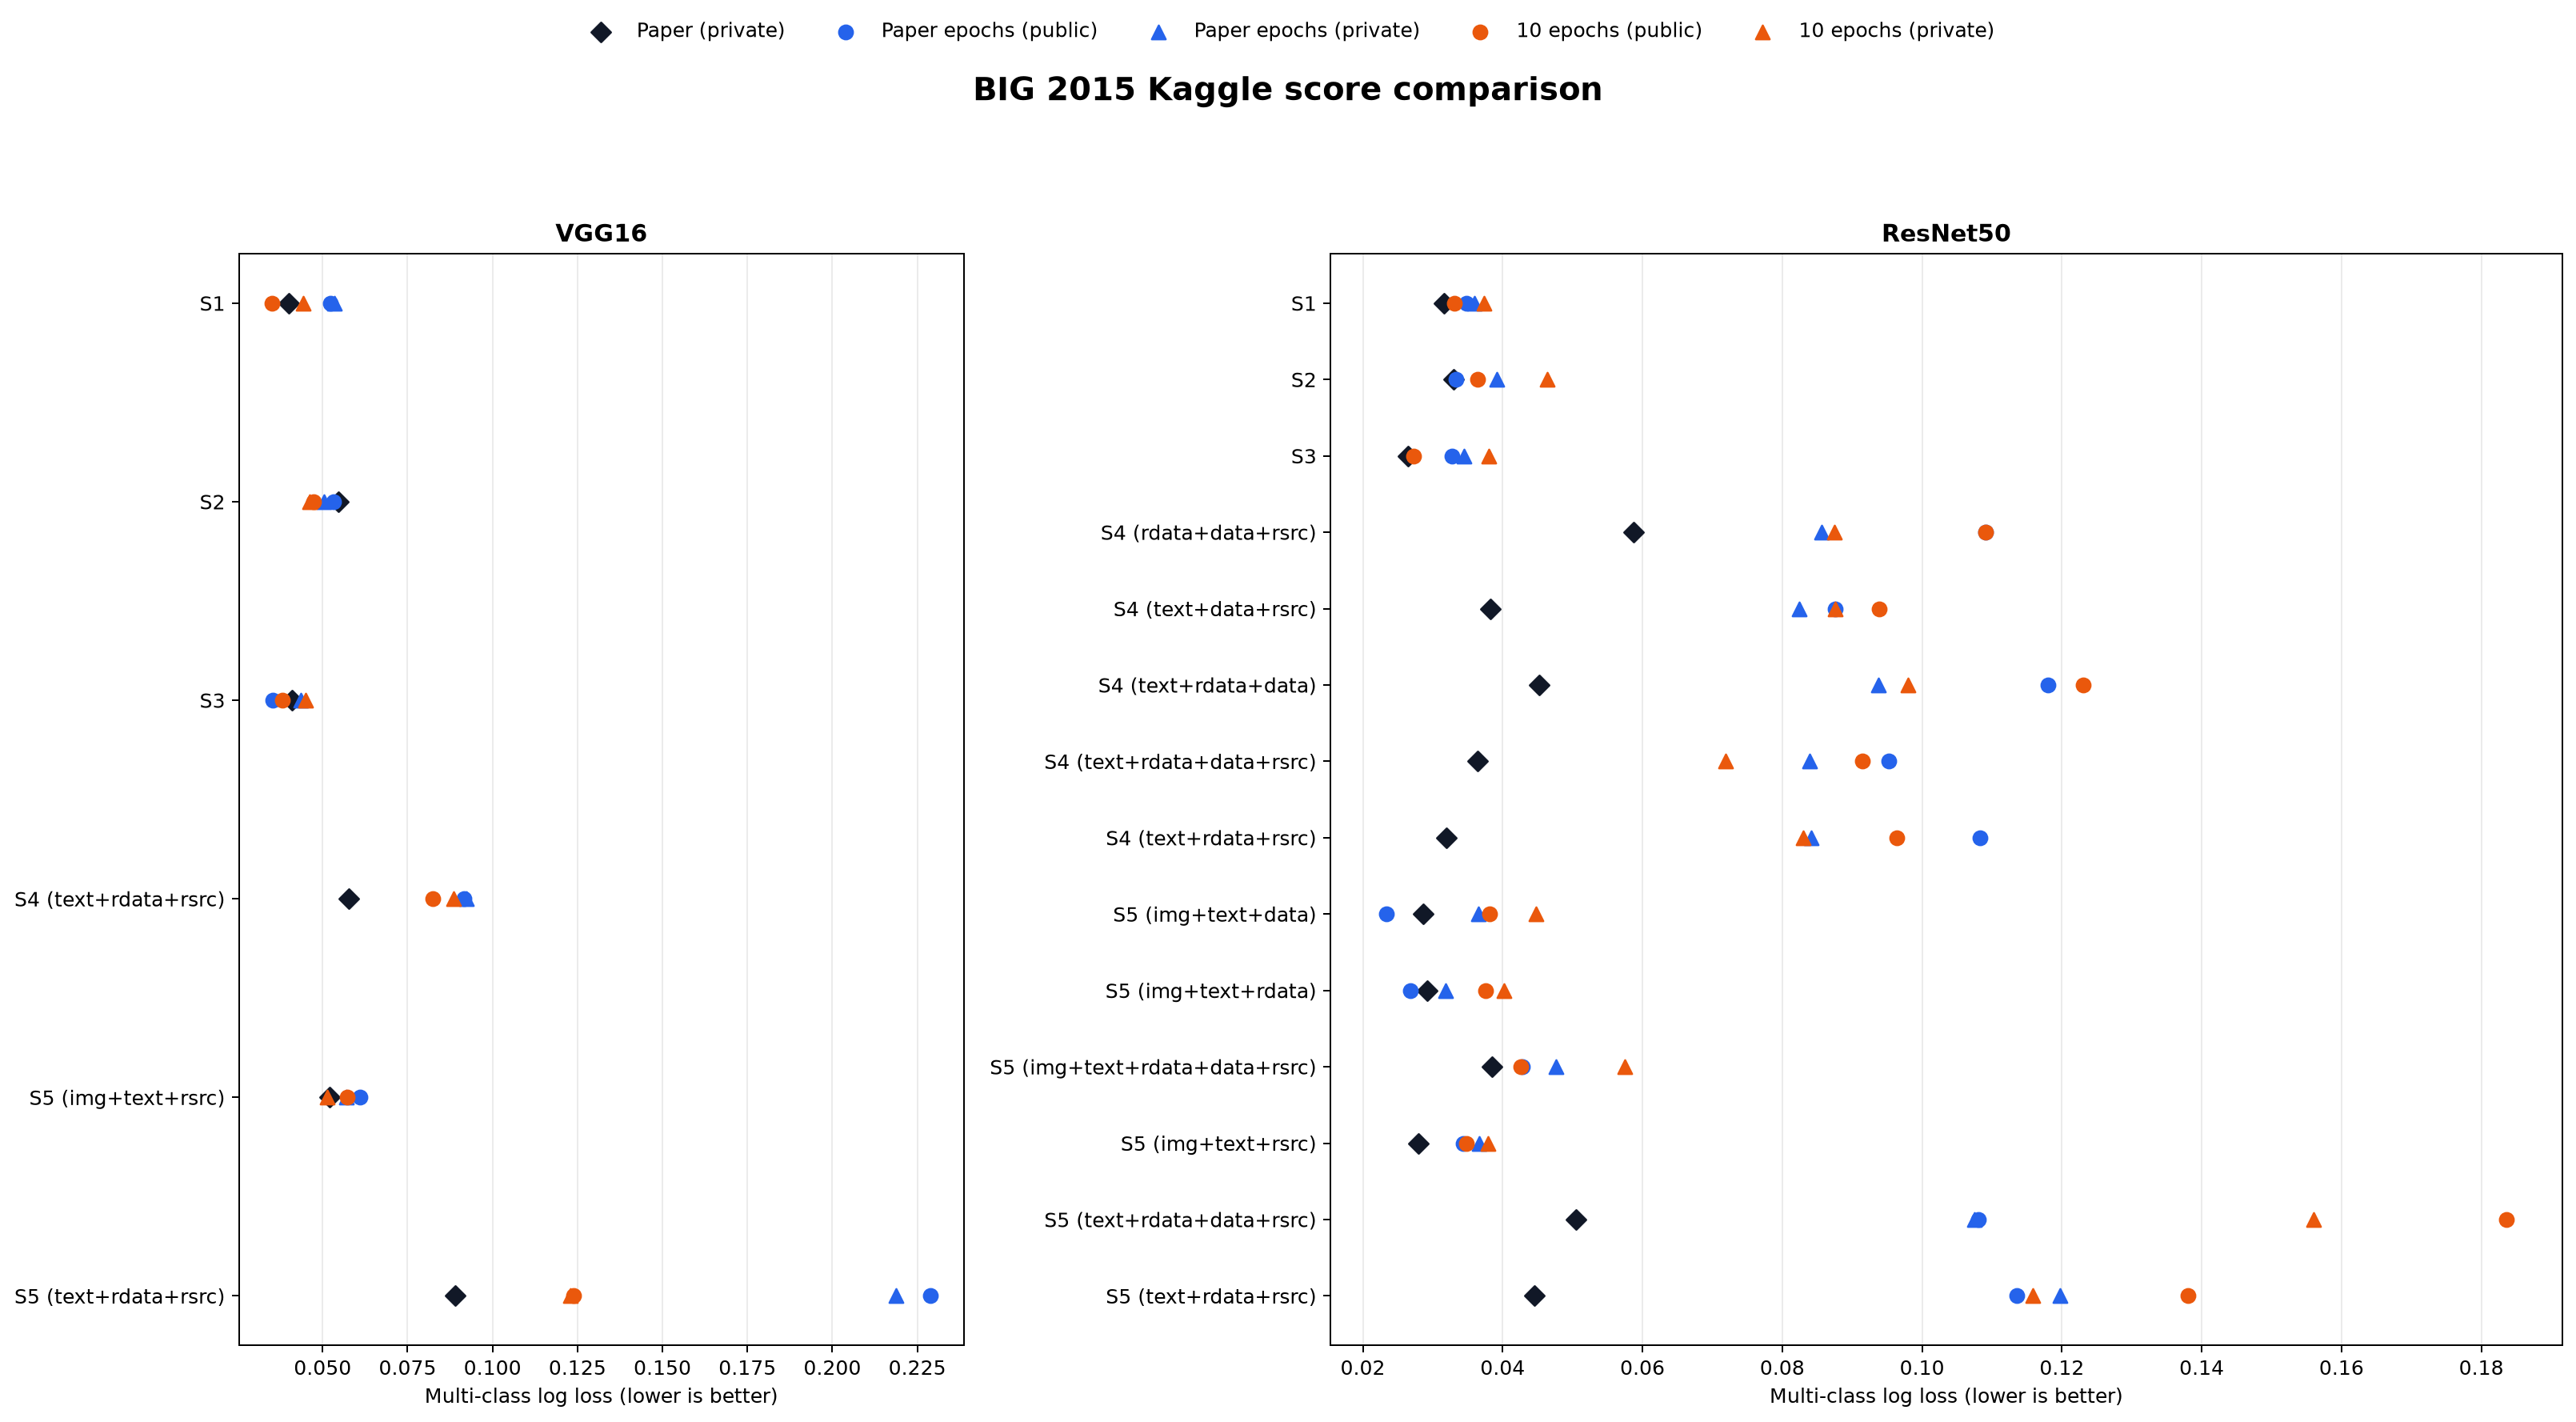
\includegraphics[width=0.95\textwidth]{figs/logloss_comparison.png}
    \caption{مقایسه زیان لگاریتمی مقاله با بازتولید ما روی \lr{BIG 2015}. لوزی سیاه نمره خصوصی گزارش‌شده مقاله است؛ نشانه‌های آبی اجرای ما با بودجه دوره مقاله و نشانه‌های نارنجی اجرای ۱۰ دوره‌ای هستند.}
    \label{fig:logloss}
\end{figure}

\subsection{تحلیل}
\paragraph{صحت آموزش بازتولید شد.} همانند مقاله، همه پیکربندی‌ها به صحت نزدیک \pct{۱۰۰} روی مجموعه آموزش رسیدند. این مشاهده تأیید می‌کند که ستون صحت آموزش در جدول ۵ مقاله واقعاً بی‌اطلاع است.

\paragraph{طرح‌های خام و \lr{Mask} همراه تصویر خام با فاصله کم بازتولید شدند.} میانگین اختلاف ما با مقاله برای شش پیکربندی \lr{S1}--\lr{S3} برابر \num{+۰٫۰۰۵۰} و برای پنج پیکربندی \lr{S5} همراه تصویر خام برابر \num{+۰٫۰۰۶۷} است. بهترین نمره خصوصی ما \num{۰٫۰۳۱۸۵} است در برابر \num{۰٫۰۲۶۵} مقاله، یعنی حدود \num{۰٫۰۰۵} بدتر. بهترین نمره عمومی ما \num{۰٫۰۲۳۴۱} از تمام اعداد جدول ۵ کمتر است، ولی چون مقاله نمره خصوصی را ملاک گرفته، مقایسه منصفانه همان ستون خصوصی است.

\paragraph{ترتیب طرح‌های عرض روی \lr{ResNet50} دقیقاً بازتولید شد.} در نتایج ما \lr{S3} با \num{۰٫۰۳۴۴۶} بهتر از \lr{S1} با \num{۰٫۰۳۶۰۱} و آن بهتر از \lr{S2} با \num{۰٫۰۳۹۱۶} است؛ همان ترتیبی که مقاله گزارش می‌کند. روی \lr{VGG16} اما ترتیب بازتولید نشد: مقاله \lr{S1} را بهترین می‌داند در حالی که در اجرای ما \lr{S3} بهترین و \lr{S1} بدترین است. این ناسازگاری، ایراد «الف» در \S\ref{sec:critique} را تقویت می‌کند: تفاوت‌های کوچک میان این طرح‌ها پایدار نیستند.

\paragraph{بزرگ‌ترین واگرایی در \lr{S4} و \lr{S5} بدون تصویر خام رخ داد.} میانگین اختلاف ما با مقاله برای شش پیکربندی \lr{S4} برابر \num{+۰٫۰۴۲۳} و برای سه پیکربندی \lr{S5} بدون تصویر خام برابر \num{+۰٫۰۸۷۴} است؛ یعنی یک مرتبه بزرگی بیش از واگرایی طرح‌های خام. این واگرایی نظام‌مند است و همه ۹ پیکربندی این دو خانواده را در بر می‌گیرد. پیامد آن مستقیماً به نتیجه‌گیری دوم مقاله می‌خورد: در اعداد مقاله \lr{S4} روی \lr{ResNet50} «مشابه» \lr{S1}--\lr{S3} است، ولی در اعداد ما دو تا سه برابر بدتر. منشأ این شکاف (سیاست کانال‌های غایب، جزئیات منتشرنشده استخراج بخش‌ها، یا نوسان اجرا) را نمی‌توان تعیین کرد؛ ولی می‌توان گفت ادعای «قطعه‌بندی به‌تنهایی کافی است» با یک بازپیاده‌سازی مستقل و وفادار به توصیف منتشرشده بازتولید نمی‌شود.

\paragraph{بودجه آموزش تعیین‌کننده نیست.} در ۸ پیکربندی از ۲۰، اجرای ۱۰ دوره‌ای نمره خصوصی بهتری از اجرای با بودجه کامل داد. هیچ الگوی نظام‌مندی به سود بودجه بیشتر دیده نمی‌شود، که با اشباع سریع صحت آموزش سازگار است.
